\documentclass[a4paper, 12pt]{report}

\usepackage[utf8]{inputenc}
\usepackage[spanish]{babel}
\usepackage{graphicx}
\usepackage{float}


\title{Influencia de la Opinión Pública en la Variabilidad de las Acciones de Tesla: Un Enfoque Predictivo}
\author{Guillermo López Gómez}
\date{\today}



\begin{document}

\maketitle

\tableofcontents
    \chapter{Resumen}
    \chapter{Introducción}
        \section{Antecedentes}
                Tesla (con razón social denomidada Tesla, Inc., TESLA SPAIN SL en España) es una empresa de origen estadounidense con domicilio social en Austin, TX.
                Es liderada por el célebre empresario Elon Musk, quien en el momento de escribir este documento ocupa el puesto de cofundador y director ejecutivo de la compañía.
                Tesla se dedica a la fabricación de vehículos eléctricos, paneles solares y baterías de almacenamiento de energía, habiendo obtenido un gran éxito en los últimos años.\\

                Con un ROE (Return on Equity) máximo del 31.78\%
                y un ROA (Return on Assets) del 17.28\%  a finales de 2022, Tesla se sitúa en el primer puesto de las empresas más rentables del sector 
                de vehículos de motor  y limpiezas, con algo 12600 millones de dólares 
                de beneficios anuales y uno de los mayores incrementos en empresas con una valoración económica similar, con 127.5\%, habiendo batido incluso 
                el incremento del Bitcoin. Esto convierte a Tesla
                en una de las empresas más atractivas para invertir en valores en los últimos años.\\

                Por su parte, Twitter es una red social de microblogging que permite a sus usuarios enviar y leer mensajes de hasta 280 caracteres llamados \textit{tweets}.
                Recientemente fue adquirida por Musk con el objetivo de mejorar la experiencia de los usuarios y promover la libertad de exresión. 
                Al ser una red social en la que los usuarios pueden expresar de manera instantánea sus opiniones sobre cualquier tema, Twitter es de especial interés y relevancia para este estudio.

        \section{Objetivos}

                
                El último objetivo de este estudio es analizar el impacto de la opinión pública en la valoración de las acciones de Tesla, 
                con el fin de predecir su comportamiento futuro y obtener una ventaja competitiva en el mercado de valores. La opinión pública es una dimensión muy difícil de medir,
                tanto por la dificultad de obtener los datos como por la subjetividad de los mismos. Al quedar la opción de realizar cualquier tipo de encuesta o cuestionario a una 
                muestra de la población descartada por la dificultad de obtener una muestra representativa y sin sesgos, además de la dificultad añadida que tendría su correspondiente análisis 
                análisis y validación, se optó por X como una base de datos en la que se pueda obtener este tipo de información.\\

        \section{Metodología}

                Para este estudio se ha optado por utilizar varios modelos de aprendizaje automático aplicados a los diferentes sets de datos obtenidos,
                siendo finalmente combinados para formar un ensemble que permita obtener una predicción más precisa y robusta.\\

                Para ello, se seguirán las diferentes fases del proceso de trabajo de ciencia de datos. Aunque se tratan más en profundidad en cada una de sus respectivas secciones,
                se resumen a continuación:

                \begin{enumerate}
                        \item \textbf{Adquisición y Caracterización:} Se obtendrán las diferentes bases de datos relevantes para el objeto de estudio y se realizará 
                        un análisis de datos exploratorio para conocer la estructura y características de cada set.
                        \item \textbf{Preprocesamiento:} Se prepararán los datos para su posterior uso en el entrenamiento y validación de los modelos de aprendizaje automático elegidos.
                        \item \textbf{Modelado:} Se entrenarán los modelos de aprendizaje automático seleccionados.
                        \item \textbf{Evaluación:} Se evaluarán los modelos elegidos con diferentes métricas.
                \end{enumerate}

                En cuanto a herramientas utilizadas, se ha optado por python como el principal lenguaje de programación, 
                utilizando notebooks de Jupyter para el análisis y entrenamiento previamente mencionados. También se utilizará
                markdown para diferentes clarificaciones en los scripts. Por último, se ha utilizado \LaTeX para la redacción de esta memoria. Las 
                diferentes herramientas específicas utilizadas y la razón de su uso están detalladas dentro de cada sección de este trabajo o en 
                los scripts del repositorio de este proyecto.\\

        \section{Limitaciones}

                Este trabajo presenta varias limitaciones causadas tanto por la naturaleza de los datos como por la metodología utilizada.
                Una de las limitaciones más importantes es la dudosa representatividad de la muestra obtenida. Existen muchos tipos de inversores en el mercado de valores,
                sin que la mayoría de ellos tengan cuenta en X. Si se toma como población toda aquella persona que invierte o tiene intención de invertir en este mercado,
                la muestra obtenida no recoge muchas de las opiniones, públicas o privadas, de instituciones o inversores ajenos a la plataforma, por lo que es más que probable 
                que la muestra tratada en este estudio no sea representativa de la población de inversores en su conjunto.\\

                Dicho esto, es innegable la contribución que tiene la red social en la opinión pública. Existen casos como el de Eli Lilly \cite{BBCNewsMundo}, en los que la plataforma puede afectar de una
                forma muy significativa en la valoración de una empresa. Por ello, ante la no existencia de bases de datos con estos datos epecíficos se decidió utilizar X como 
                alternativa. Inicialmente, se pensaba utilizar la interfaz de desarrollo (API por sus siglas en inglés) de la empresa para obtener todos aquellos post (también conocidos como \textit{tweets} antes de la compra de Twitter por parte de Musk). Sin embargo,
                tras el cambio de director ejecutivo, se decidió que esa API pasaría a ser de pago. Como el estudio no tiene ningún tipo de presupuesto económico al ser un trabajo de final de curso,
                se tuvo que pensar en una alternativa gratuita.\\

                Al ser Tesla una empresa muy conocida y con un gran número de seguidores, existen varios datasets públicos con tweets relacionados con la empresa. Aunque esta es una alternativa gratuita,
                limita en gran medida el alcance de este estudio por diferentes razones. En primer lugar y más importante, no se puede garantizar que los tweets obtenidos sean representativos de la opinión pública,
                ya que no se puede garantizar que la muestra de tweets obtenida sea representativa de la población. En segundo lugar, el dataset elegido es muy limitado en términos temporales, al abarcar
                un periodo de 31 semanas. En una futura revisión de este trabajo, se podría obtener acceso a la API de X para obtener un dataset más completo y representativo.\\

        \section{Motivación}

                La razón principal de la existencia de este trabajo es el afán por poder obtener una nueva ventaja competitiva en el mercado de valores.
                Este mercado puede llegar a ser muy volátil y difícil de predecir, debido a la gran cantidad de factores y dimensiones que hay que tener en cuenta a la hora de estimar
                el valor de una acción.

                De forma más personal, tengo un gran interés por el mundo de las finanzas y la inversión. Creo que este trabajo puede ser una gran oportunidad
                para poder profundizar más en este sector y conocer cómo funciona este fenómeno. En un mercado tan competitivo como el actual, cualquier ventaja competitiva es bienvenida,
                estando ya la mayoría de indicadores financieros muy estudiados. Por ello, tomar una aproximación más holística y menos tradicional, utilizando 
                técnicas de aprendizaje automático, puede ser una gran oportunidad de aprendizaje.\\

        \section{Alcance y Aplicaciones}

                        
                Este trabajo cuenta con un alcance muy limitado, condicionado sobretodo por la falta de acceso a la api de X, y la asunción de que la muestra obtenida de la plataforma es representativa de la sociedad en su conjunto.


                Entre sus potenciales aplicaciones, podría utilizarse el modelo propuesto en este estudio como una base de sistema de trading automático,
                en el que se tomen decisiones de compra y venta de acciones de Tesla en función de la predicción de su valor.\\


    \chapter{Análisis Exploratorio de Datos}

        \section{Adquisición de Datos}

                Para dar solución al problema propuesto, se necesitan dos fuentes de datos diferentes. Primeramente, es necesario obtener un dataset de la opinión pública sobre tesla
                 que sea representativo de la población. Por otra parte, es necesario obtener una base de datos de la que se extraigan los datos financieros de Tesla.\\

                Para la obtención de la base de datos de la opinión pública, se optó primeramente por utilizar la API de X. Dentro de la plataforma, se puede referenciar a las 
                acciones de cualquier empresa que cotice en un mercado de valores con el símbolo \textit{\$}. Así, al buscar posts con el identificador \textit{\$TSLA},
                se podrían obtener posts fuertemente relacionados con los valores de tesla. Sin embargo y como se mencionó en la sección anterior, la API de X pasó a ser de pago 
                a los pocos meses del cambio de director ejecutivo, por lo que no se pudo utilizar esta vía.\\

                Por ello, se optó por utilizar un dataset público de Kaggle \cite{shafaghi2022}. Este dataset contiene 31 semanas de tweets que contienen el símbolo \textit{\#Tesla}.
                Aunque no es una muestra representativa de la población, es una alternativa gratuita que permite obtener una idea de la opinión pública sobre Tesla.\\

                Para la obtención de datos financieros de la empresa, se utilizó la API de Yahoo Finance, que permite obtener este set de forma muy sencilla.\\

        \section{Caracterización de Datos}

                En esta sección se realizará un análisis exploratorio de datos de los diferentes datasets obtenidos.
                El análisis exploratorio de datos (EDA por sus siglas en inglés) es una técnica de análisis de datos que permite investigar un conjunto de datos y sus características, así como estructura.
                Se apoya en diferentes técnicas estadísticas y de visualización de datos para obtener una mejor idea de cómo proceder hacia su manipulación y modelado. Permite detectar anomalías, probar
                hipótesis y descubrir patrones de interés ocultos. \\

                En el caso de este estudio, se han utilizado diferentes técnicas para analizar ambas bases de datos, al tratar con datos de típo numérico y de texto, en el dataset de 
                datos financieros y de tweets respectivamente.\\
                
                \subsection{Dataset de Tweets de Tesla}
                        Con un nombre de archivo \textit{ tesla\_tweets.csv } y 57.2 MB de peso, este dataset contiene 31 semanas de tweets que contienen el símbolo \textit{\#Tesla}.
                        Contiene en total 152.000 tweets, con 5 columnas diferentes, todas ellas de tipo \textit{string}. Cada columna hace referencia a una variable diferente:\\

                        \begin{itemize}
                                \item \textbf{Date \& Time:} Fecha de publicación del tweet. Aunque legible, no se encuentra en ningún formato conocido por el autor, por lo que se dejará que la biblioteca pandas infiera la fecha en el preprocesamiento.
                                \item \textbf{Profile Picture Link:} Enlace a la imagen de perfil del usuario que publicó el tweet. No es de mucho interés para el análisis, por lo que se eliminará en la etapa de preprocesamiento.
                                \item \textbf{Twitter ID:} Handle del usuario que publicó el tweet. No es de mucho interés para el análisis, por lo que también se eliminará en la etapa de preprocesamiento.
                                \item \textbf{Tweet Text:} Contenido del tweet en cuestión. Es la variable de más importancia de cara al análisis.
                                \item \textbf{Tweet Link:} Enlace al tweet referenciado. Aunque no es de mucho interés para el análisis, se puede llegar a utilizar para identificar de forma unívoca cada post, por lo que se mantendrá en el dataset.
                        \end{itemize}

                        Una vez estudiada la estructura del dataset y haber eliminado las columnas no deseables, se procede a realizar un 
                        análisis de contenido del mismo, especialmente de la columna \textit{Tweet Text}.\\

                        \subsubsection{Columna de Tweet Text}

                        Como ha sido mencionado anteriormente, esta columna es la única relevante para el análisis de sentimiento de los post. Al ser una columna de tipo \textit{string},
                        tuvieron que utilizarse técnicas diferentes a las convencionales de análisis numérico para poder obtener una idea de su contenido.\\

                        Inicialmente se obtuvo la longitud de cada tweet en caracteres en palabras, y se visualizó la distribución de los mismos, utilizando 
                        tanto un gráfico con \textit{bins} como una función calculada con el Kernel Density Estimate (KDE).\\

                        \begin{figure}[H]
                                \centering
                                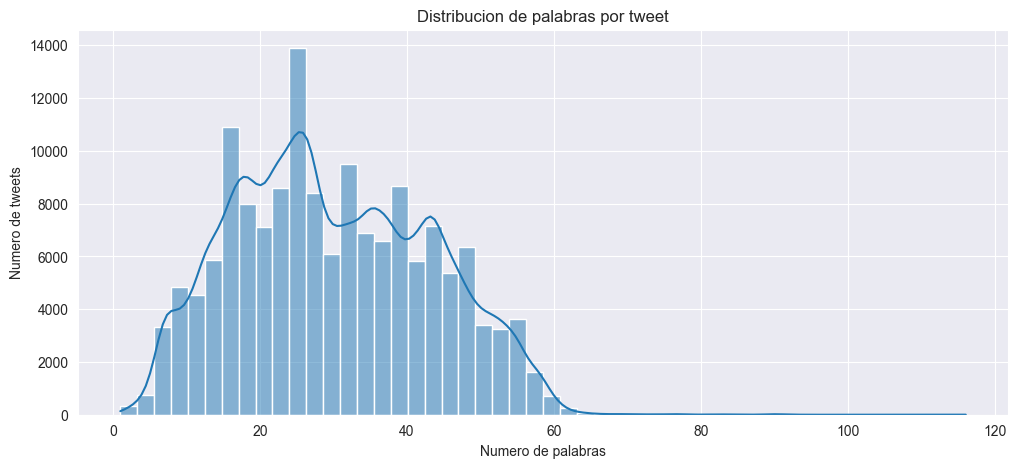
\includegraphics[width=0.8\textwidth]{resources/images/words_per_tweet_distr.png}
                                \caption{Distribución del número de palabras por cada tweet.}
                                \label{fig:word_count_distribution}
                        \end{figure}

                        Como se puede observar en la figura \ref{fig:word_count_distribution}, la mayoría de tweets tienen entre 20 y 40 palabras, con una media de 29.95 palabras por tweet (\(\bar{\mu} = 29.9512\)) y una desviación típica de 13.32 (\(\sigma = 13.3260\)).\\

                        \begin{figure}[H]
                                \centering
                                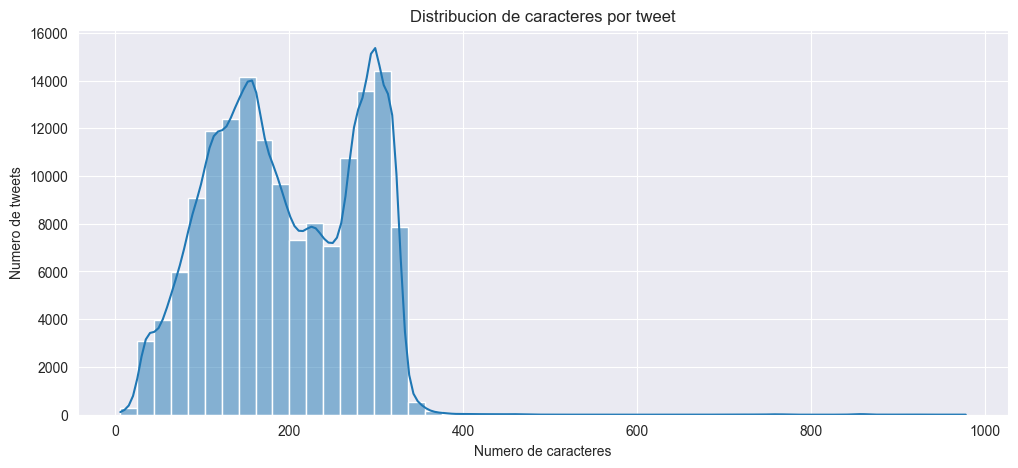
\includegraphics[width=0.8\textwidth]{resources/images/character_per_tweet_distr.png}
                                \caption{Distribución del número de caracteres por cada tweet.}
                                \label{fig:character_count_distribution}
                        \end{figure}

                        Por otra parte, la distribución del número de caracteres por tweet se puede observar en la figura \ref{fig:character_count_distribution}. En este caso, la mayoría de tweets tienen entre 100 y 200 caracteres, con una media de 196.73 caracteres por tweet (\(\bar{\mu} = 196.7343\)) y una desviación típica de 72.5 (\(\sigma = 84.9298\)).\\

                        Se comprobó, tal como se puede ver en la figura \ref{fig:character_count_distribution}, 
                        que existen tweets con más de 280 caracteres, que era el límite de caracteres en un post antes de que Musk
                        eliminase el limite para usuarios de Twitter Blue en 2023. Esto no debería ser posible, por lo que se comprobó la exitencia de este tipo de tweet.\\

                        Se obtuvieron resultados de cerca de 35.000 tweets con más de 280 caracteres, lo que representa alrededor de un 23\% del total de tweets.
                        El tweet con mayor longitud contaba con 950 caracteres, superando con creces el límite mencionado. Al verificar la naturaleza de este tipo de tweets,
                        se descubrió que todos ellos contenían un gran número de menciones a otros usuarios, que no se contaban como caracters adicionales y provocaba que el número de caracteres se incrementase de forma considerable. Como 
                        estas menciones no poseen valor explicativo para el modelo, serán limpiadas en la etapa de preprocesamiento\\

                        \begin{figure}[H]
                                \centering
                                \includegraphics[width=0.8\textwidth]{resources/images/word_cloud.png}
                                \caption{Wordcloud de las palabras más frecuentes en el dataset.}
                                \label{fig:wordcloud}
                        \end{figure}

                        Finalmente, se obtuvo una lista con las palabras más frecuentes en el dataset, obteniendo un \textit{word cloud} como el de la figura. Se limpiaron previamente símbolos y caracteres especiales propios de la plataforma como ReTweets o menciones a otros usuarios,
                         además de stopwords que se obtuvieron de la biblioteka \textit{ntlk}.\\


                \subsection{Dataset de Datos Financieros de Tesla}

                        Como fue mencionado anteriormente, esta base de datos fue obtenida utilizando la API de Yahoo Finance. Con un nombre de archivo \textit{tesla\_stocks.csv} y un muy inferior peso al anterior dataset de 16 KB,
                        contiene 31 semanas de datos financieros de la cotización de Tesla en el mercado de valores. Contiene un total de 150 observaciones, con 7 columnas diferentes:\\

                        \begin{itemize}
                                \item \textbf{Date:} Fecha de cotización del valor de la empresa. Se encuentra en tipo datetime.
                                \item \textbf{Open:} Valor de la acción al inicio del día. Se encuentra en tipo float.
                                \item \textbf{High:} Valor máximo de la acción durante el día. Se encuentra en tipo float.
                                \item \textbf{Low:} Valor mínimo de la acción durante el día. Se encuentra en tipo float.
                                \item \textbf{Close:} Valor de la acción al cierre del día. Se encuentra en tipo float.
                                \item \textbf{Adj Close:} Valor de la acción al cierre del día, ajustado por dividendos y splits. Se encuentra en tipo float. Esta columna puede llegar a ser problemática porque en muchos casos no hay ajuste y los valores son los mismos que los de la columna anterior.
                                \item \textbf{Volume:} Volumen de acciones negociadas durante el día. Se encuentra en tipo int.
                        \end{itemize}

                        Tras analizar la estructura del dataset, se utilizó la biblioteca \textit{summarytools} para obtener un resumen muy completo del dataframe.
                        Esta biblioteca no se pudo utilizar para el caso anterior al ser sólo compatible con datos de tipo numérico.\\

                        \begin{figure}[H]
                                \centering
                                \includegraphics[width=0.8\textwidth]{resources/images/stock_stats.png}
                                \caption{Resumen del dataset utilizando la biblioteca \textit{summarytools}.}
                                \label{fig:summarytools}
                        \end{figure}

                        Gracias a esta tabla, se comprueba que no existen nulos ni valores duplicados en el dataset, además de poder visualizar
                        valores máximos y mínimos, media y desviación estándar y distribuciones de cada columna.\\

                        De este resumen se puede extraer un dato preocupante. Ambas columnas de precios de cierre (ajustado y no ajustado) parecen tener la misma
                        distribución, así como indicadores de centralidad y dispersión idénticos. Esto es especialmente problemático al ser el precio de cierre 
                        sin ajustar nuestra variable a predecir, ya que si no se elimina la columna le estaríamos introduciendo ya la variable objetivo al modelo. Se verificó si existían datos
                        distintos entre las columnas, para lo que se obtuvo que ambas eran completamente idénticas en todas las observaciones. Por ello, la columna \textit{Adj Close} será
                        eliminada en el preprocesamiento de datos. \\

                        Por otra parte, también se advirtió una incongruencia entre el número de observaciones y el número de días que hay en el periodo designado.
                        Mientras el periodo entre el 11 de abril de 2022 y el 11 de Noviembre es de 214 días, el número de observaciones es de 150. Tras una investigación cualitativa más profunda del 
                        mercado de valores del que se ha extraído el dataset, se descubrió que el mercado de valores no abre los fines de semana ni festivos, por lo que el número de observaciones se corresponde con 
                        el número de días laborables en el periodo de tiempo designado.\\

                        Seguidamente, se graficaron los valores de cada variable a lo largo del tiempo.

                        \begin{figure}[H]
                                \centering
                                \includegraphics[width=0.8\textwidth]{resources/images/stocks_time_series.png}
                                \caption{Evolución de los valores de las acciones de Tesla a lo largo del tiempo.}
                                \label{fig:stocks_time_series}
                        \end{figure}

                        Al analizar esta figura, resalta la gran similitud que tienen todas las gráficas, menos la del volumen de acciones negociadas.
                        Esto puede significar que existe una gran correlación entre las variables, lo que puede ser problemático para el modelo.\\

                        \begin{figure}[H]
                                \centering
                                \includegraphics[width=0.8\textwidth]{resources/images/stock_correlation_matrix.png}
                                \caption{Matriz de correlación de las variables del dataset.}
                                \label{fig:stocks_corr}
                        \end{figure}

                        Para comprobar esta hipótesis, se obtuvo la matriz de correlación de las variables, que se puede observar en la figura \ref{fig:stocks_corr}.
                        Se observa que existe una correlación extremadamente fuerte entre todas las variables numéricas, menos con el volumen de acciones negociadas.
                        Se ha deducido que esto se debe a que estas variables son todas indicadores de la misma cosa, el precio de la acción. Si el precio del valor
                        está sufriendo una tendencia alcista, es esperable que todas estas variables se incrementen en el mismo momento.\\
                        
                        Por otra parte, el volumen de acciones es un indicador completamente, por lo que no sigue esta tendencia.Se aprecia una correlación negativa significativa en algunos casos
                        (-0.46 con el precio más bajo del día), que se puede explicar al aplicar teoría financiera al problema. Si la correlación entre el volumen de acciones negociadas y el precio de la acción es negativa, 
                        esto puede ser una señal de debilidad, al no estar los inversores seguros de la tendencia del precio o que existe un alto interés de venta del valor.\\
                        
    \chapter{Preprocesamiento de Datos}

                El preprocesamiento de datos es un conjunto de tareas y técnicas aplicadas a los datos de entrenamiento y validación de un modelo de machine learning. El objetivo es 
                mejorar la calidad y poder predictivo de los datos, siendo necesario para ello limpiar, transformar y estructurar los datos de forma que estos sean más útiles para el algoritmo de machinelearning a utilizar.
                A continuación, se llevará a cabo la limpieza y preprocesameinto de los datos tratados en la caracterización.

                \section{Dataset de Tweets de Tesla}

                        Tras haber obtenido extensa información valiosa sobre el dataset en la etapa de caracterización, 
                        se procede a la preparación de los datos para ser etiquetados por el autor del trabajo. Se procesó
                        sobretodo la columna de texto, ya que es la única que contiene información relevante para el modelo de análisis de sentimiento.\\

                        Para obtener las cadenas de texto más significativas y con mayor poder de predicción para el modelo es necesario 
                        realizar unalimpieza de todos aquellas palabras, caracteres y otros símbolos que no aportan información relevante.
                        Es necesario notar además la dificultad añadida que presentan las cadenas de texto tratadas en este trabajo, ya que
                        los tweets son textos cortos, con gran número de abreviaciones y errores ortográficos, pero sobretodo por el uso de 
                        funcionalidades propias de la plataforma, como menciones, hashtags o retweets. Para ello, se utilizó la librería \textit{tweet-preprocessor}\cite{tweet-preprocessor}. Con ella, se eliminaron emojis, menciiones, palabras reservadas de twitter, emojis de texto, hashtags, urls y números.\\

                        Además, es necesario tener en cuenta que el modelo de análisis de sentimiento a utilizar solo aceptará texto en idioma inglés,
                        por lo que es necesario eliminar todos aquellos tweets que no estén escritos en esta lengua. Para ello se utilizó la
                        librería \textit{langdetect} \cite{langdetect}, que permite detectar el idioma de un texto utilizando la librería de detección de lenguas de Google.\\

                        Habiendo filtrado los tweets en inglés y haber eliminado todos aquellos caracteres y palabras no deseados, se eliminaron también signos de puntuación restantes 
                        y las stopwords de la lengua inglesa, utilizando la librería \textit{nltk}.\\

                        Por último, como fue constatado en la caracterización de datos, existen días en los que los mercados no están abiertos.
                        Esto puede llegar a ser problemático para el modelo, ya que pueden existir tendencias en un hiato de varios días que no serían capturadas por el modelo. Para su simplificación,
                        se ha optado por eliminar todos aquellos tweets que no se encuentren en los días recogidos en el dataset de valores de la empresa, pero
                        sería interesante explorar esta posibilidad en una futura revisión de este trabajo.\\

                \section{Dataset de Datos Financieros de Tesla}

                        
                        

                        

    \chapter{Selección y Entrenamiento de Modelos}
    \chapter{Evaluación de Modelos}
    \chapter{Gestión del proyecto}
    \chapter{Conclusiones}
    \bibliographystyle{unsrt}
    \bibliography{references}
    \chapter{Anexos}


\end{document}


